%! Author = denis
%! Date = 15/09/2025

% Slide 10
\begin{frame}{Conceitos fundamentais sobre IoT}
    Definição:
    
    \begin{columns}[c]
        \column{0.55\textwidth}
        \small
        \textit{"IoT é a conexão de objetos físicos à internet, permitindo que eles coletem, troquem e processem dados, gerando inteligência e novas oportunidades de negócio."}
        
        \column{0.45\textwidth}
        \begin{center}
            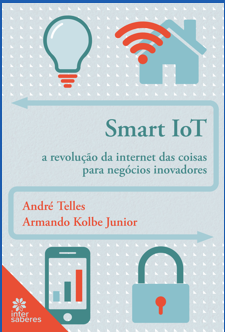
\includegraphics[width=0.35\textwidth]{images/smart_iot_book.png}
            \label{fig:Smart IoT: a revolução da internet das coisas para negócios inovadores}
        \end{center}
    \end{columns}
    
    \begin{columns}[c]
        \column{0.55\textwidth}
        \small
        \textit{"uma filosofia de desenvolvimento em que dispositivos físicos (com sensores e atuadores) se conectam à internet e interagem com outros sistemas e ambientes."}

        \column{0.45\textwidth}
        \begin{center}
            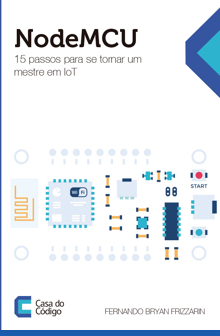
\includegraphics[width=0.35\textwidth]{images/node_mcu_book.png}
            \label{fig:NodeMCU: 15 passos para se tornar um mestre em Iot}
        \end{center}
    \end{columns}
\end{frame}

    